
In the previous chapter we regularized the value estimate by adding a regularization term to the objective(target). In this chapter we explore explicitly averaging the value estimate using exponential smoothing.

\begin{abstract}

In sequential modelling, exponential smoothing is one of the most widely used techniques to maintain temporal consistency in estimates. In this work, we propose Recurrent Learning, a method that estimates the value function in reinforcement learning using exponential smoothing \emph{along the trajectory}. We establish its asymptotic convergence properties under some smoothness assumption on the reward.  The proposed algorithm yields a natural way to learn a state dependent emphasis function that selectively learns to emphasize or ignore states based on trajectory information. We demonstrate the potential for this selective updating on a partially observable domain and several continuous control tasks.

\end{abstract}

\section{Introduction}
Reinforcement Learning is a mathematical framework designed to model sequential decision making. It is used to solve a wide range of control tasks ranging from video games \cite{vinyals2017starcraft,mnih2013playing,mnih2016asynchronous} to robotics \cite{kober2013reinforcement,abbeel2010autonomous}. It is also used in many real-life applications such as hydro control \cite{grinberg2014optimizing} and power grid management \cite{franccois2016deep}.

However, reinforcement learning algorithms suffer from several issues. In particular, we describe two issues that Recurrent Learning attempts to mitigate. The first one considers the \emph{variance of the value estimates through the trajectory}. Consider a hypothetical scenario in which a person is driving a car at a high speed. Its behavior needs to be temporally coherent. If the driver wants to change lane, there needs to be a continuous smooth decision making process. For the policy of the driver to be coherent, its value function needs to be temporally smooth. Most algorithms make a decision at every time step without necessarily \emph{explicitly} enforcing temporal coherence nor considering previous decisions. This can lead to erratic and temporally inconsistent behaviors, particularly in tabular and discrete settings. The second issue considers the limited capacity of the brain to process information and make decision. Bounded rationality argues that human brain has a limited capacity to learn and can't store all the information. In this work we argue that the capacity to ignore or emphasize chosen state is a key component for the success of decision making algorithms.  
To summarize, this work proposes a method that attempts to address the following two aspects. 1) Minimization of the variance of the estimates through the \emph{trajectory}. 2) Learn a mechanism that emphasizes and de-emphasizes updates on relevant states.\\
Exponential smoothing \cite{gardner1985exponential} is one of the most widely used technique to reduce the variance of point estimates using \emph{previous observations}.
\begin{equation}
\begin{split}\label{smoothing}
    x_t &= \param s_t + (1-\param) x_{t-1}
\end{split}
\end{equation}
where $s_t$ is a signal, $x_t$ the averaged signal at time step $t$ and $\param$ a smoothing factor.
In time series data it is used to approximate the mean of a stream of data. This kind of smoothing has various names \cite{polyak1992acceleration,kingma2014adam} depending on the field it is used in.  Most quantities in reinforcement learning (Q values, state values, actions, etc) are estimated as point estimate ignoring previous estimates from the trajectory. We propose to use exponential smoothing in reinforcement learning on the trajectory. In other words, we propose to smooth the estimate of a state $s_t$ using the estimates of states $s_i$ that occur earlier in the trajectory ($i\geq t$). Intuitively, states that are temporally close to each other should have similar value.\\
However, exponential averaging can be biased if a sharp change(non-stationarity) is encountered in the trajectory, like falling off a cliff. To alleviate this issue a common technique used is to set $\param_t$ the exponential smoothing factor as a state or time dependent. In Recurrent Neural Networks, it is possible to view LSTM \cite{hochreiter1997long} and GRU \cite{chung2014empirical} as several non linear exponential smoothing functions. The key ingredient is the gating mechanism(state dependent $\param_t$) used to update the hidden cell. The capacity to ignore information allows the cell to focus only on important information. This can also be found in semi-iterative method used to solve linear system of equations. \cite{golub1961chebyshev} finds the optimal $\param_t$ using Chebyshev polynomials. In this work we explore a new method that attempts to learn a state dependent smoothing factor $\param$. We show how it relates to existing methods and exploits similar properties such as emphatic TD \cite{sutton2016emphatic,mahmood2015emphatic}. 
The contributions of the paper are as follows:
\begin{itemize}
    \setlength\itemsep{0.1em}
    \item Propose a new way to estimate value function in reinforcement learning by exploiting the estimates along the trajectory.
    \item Provide asymptotic convergence guarantee in the tabular setting under some smoothness assumption.
    \item Derive a learning rule for a state dependent $\param$.
    \item Perform a set of experiments in tabular and continuous settings to evaluate its strengths and weaknesses.
\end{itemize}

\section{Technical Background}
A Markov Decision Process (MDP), as defined in \cite{puterman2014markov}, consists of a discrete set of states $\s$, a transition function $\p : \s \times \A \times \s \mapsto [0,1]$, and a reward function $\RE : \s \times \A \mapsto \R$. On each round $t$, the learner observes current state $s_t\in\s$ and selects action $a_t\in\A$, after which it receives reward $r_t = \RE(s_t,a_t)$ and moves to a new state $s_{t+1}\sim \p(\cdot|s_t, a_t)$. We define a stationary policy $\pol$ as a probability distribution over actions conditioned on states $\pol : \s \times \A \mapsto [0,1]$, such that $a_t \sim \pol(\cdot|s_t)$. 
When performing policy evaluation, the goal is to find the optimal value function $V^{\pol}$ that estimates the discounted expected return of policy $\pol$ at a state $s\in\s$, $V^{\pol}(s) =\expect_{\pol}[\sum_{t=0}^{\infty} \gamma^t \RE_{t+1} | s_0 = s]$, with discount factor $\gamma \in [0,1)$. In this paper we only consider policy evaluation and simplify the notation: $r(s_t)=r(s_t,a_t)$.

In practice $V^{\pol}$ is approximated using Monte Carlo rollouts \cite{suttonreinforcement} or TD methods \cite{sutton1988learning}. In reinforcement learning the aim is to find a function $V_\theta: \mathbb{S} \rightarrow \mathbb{R}$ parametrized by $\theta$ that approximates $V^{\pol}$. We can fall back to the tabular setting by representing the states in a one hot vector form with $\theta \in \mathbb{R^{|\mathbb{S}|}}$. The goal is to find a set of parameters $\theta$ that minimizes the squared loss:
\begin{equation}\label{simple_loss}
    \mathcal{L}(\theta) = \expect_{\pol} [(V^{\pol} - V_\theta)^2]
\end{equation}
which yields the following update by taking the derivative with respect to $\theta$:
\begin{equation}
    \theta_{t+1} = \theta_t + \alpha (V^{\pol}(s_t) - V_{\theta_t}(s_t)) \nabla_{\theta_t} \Vt(s_t)
\end{equation}
where $\alpha$ is a learning rate.\\
In the tabular setting, convergence is usually proven by casting the learning algorithm as a stochastic approximation \cite{tsitsiklis1994asynchronous,borkar2009stochastic,borkar2000ode} of the form:
\begin{equation}\label{stoch}
    \theta_{t+1} = \theta_t + \alpha( \T \theta_t  - \theta_t + w(t)) 
\end{equation}
where $\T: \mathbb{R^{|\mathbb{S}|}} \rightarrow \mathbb{R^{|\mathbb{S}|}}$ is a contraction operator and $w(t)$ is a noise term. 
As an example, TD(0) is known to converge to the fixed point of the bellman operator \cite{sutton1988learning}:
\begin{equation}
\begin{split}
    \T \Vt(s_t) &= \expect_{s_{t+1} \sim \pol} [r(s_t) + \gamma \Vt(s_{t+1})]\\
\end{split}
\end{equation}
However, in practice we have access to a noisy version of the operator $\widetilde{\T}$ due to sampling process hence the noise term $w(t)$:
\begin{equation}
    w(t) = r_t + \gamma \Vt (s_{t+1}) - \expect_{s_{t+1} \sim \pol} [r + \gamma \Vt(s_{t+1})]
\end{equation}
%COMMENT(pierre-luc) : I would merge this section with the above. Both sections are pretty small and there is no need to separate them as subsubsections.

\section{Recurrent Learning in Reinforcement Learning}
\label{RLRL}
In this work, we propose to estimate the value function using the estimates along the trajectory. The value of a state $s$ at time step $t$ is given by:
\begin{equation}
\label{value}
\begin{split}
    \vr(s_t) &= \param_t \Vt(s_t) + (1 - \param_t) (\vr(s_{t-1})) \\ 
\end{split}
\end{equation}
where $\vr$ is an exponential smoothing of $\Vt$. $\vr$ is a function parametrized by $\theta$ and $\param$. We consider $\param$ to be fixed for each state in this section and relax the assumption later. For a given set of state dependant $\param(s_t) = \param_t$, the goal is to find a set of parameters $\theta$ minimizing,
\begin{equation}\label{loss_beta}
    \text{min}_{\theta} \mathcal{L}(\theta) = \text{min}_{\theta} \expect_{\pol} [(V^{\pol} - \vr)^2]
\end{equation}
In contrast to traditional methods that attempts to minimize Eq. \ref{simple_loss} we explicitly enforce temporal consistency by finding $\theta$ that minimizes Eq. \ref{loss_beta}.
By taking the derivative with respect to Eq. \ref{loss_beta} we obtain the following update:
\begin{equation}
\begin{split}
    \theta &= \theta + \alpha \delta_t  \nabla_{\theta} \vr (s_t) \\
\end{split}
\end{equation}
where $\delta_t = V^{\pol}(s_t) - \vr(s_t)$.
 The gradients of $\vr$ can be expressed in a recursive form:
\begin{equation}
    \nabla_{\theta} \vr (s_t) = \param_t \nabla_{\theta} \Vt + (1-\param_t) \nabla_{\theta} \vr (s_{t-1})
\end{equation}
For computational reason, it is possible to approximate the gradient $\nabla_{\theta}\vr (s_{t})$ using a recursive \emph{eligibility} trace:
\begin{equation}
\label{trace}
    e_t = \param_t \nabla_{\theta} \Vt (s_t) + (1-\param_t) e_{t-1}
\end{equation} 
The potential bias induced by this approximation are discussed later in the paper.
We present Recurrent Temporal Difference(RTD) in Algorithm \ref{RTD}.
\begin{algorithm}[H]
\caption{Recurrent Temporal Difference, RTD(0)}
\begin{algorithmic}[1]
    \label{RTD}
    \STATE Input: $\pi$,$\param$,$\gamma$,$\theta$
    \STATE Initialize: $\vr(s_0) = \Vt(s_0)$ and $e_0 = \nabla_{\theta} \Vt(s_0)$
    \STATE Output: $\theta$
    \FORALL{t}
        \STATE Choose $a \sim \pi(s_t)$
        \STATE Take action $a$, observe $r(s_t),s_{t+1}$
        \STATE $\vr(s_t) = \param_t \Vt(s_t) + (1-\param_t) (\vr (s_{t-1})$
        \STATE $e_t = \param_t \nabla_{\theta} \Vt(s_t) + (1-\param_t) e_{t-1}$
        \STATE $\delta_t = r(s_t) + \gamma \Vt(s_{t+1}) - \vr(s_t)$
        \STATE $\theta = \theta + \alpha \delta_t e_t $
    \ENDFOR
\end{algorithmic}
\end{algorithm}
In practice, $\vr(s_0)$ is initialized with the value of the first state $\Vt(s_0$). We can understand our algorithm better when we intuitively interpret its effect in the \emph{extreme cases} ($\param=\{0,1\}$). We consider TD(0) in a tabular setting for simplicity. First, consider a state $s_t$ where $\param(s_t) = 0$. The value of this state is frozen at the initialization point and is never updated. This is because the trace as defined in Eq. \eqref{trace} is $e_t = e_{t-1}$ making such a state \emph{ineligible} for the update. The error received at this state is used to update the previous states as per their \emph{eligibility} in $e_{t-1}$. This means that for a state $s_t$ with $\param(s_t)=1$, $\Vt(s_t)$ is updated at every time step $t+n$ until another state with $\param(s_{t+n}) = 1$ is encountered.

For any $i \leq t$ where $\param_i \in (0,1]$, it is possible to express $\vr(s_t)$ as:
\begin{equation}
\begin{split}\label{decompose}
    \vr(s_t) &= \Vt(s_i) - \Delta_t(s_i) \\
    \Delta_t(s_i) &= (1-C_t(s_i))(\Vt(s_i) - \widetilde{V}_t(s_i) ) 
\end{split}
\end{equation}
where $C_t(s_i) = \param_i \prod_{p=i+1}^t (1-\param_p)$, $\widetilde{V}_t(s_t)$ is a convex combination of all $\Vt$ encountered in the trajectory except $\Vt(s_i)$ weighted by their respective contribution($\param$) to the estimate $\vr(s_t)$. For example, if we consider updating $\Vt(s_2)$ at $t=3$ and have the following $\param_1 = 0.9,\param_2 = 0.1,\param_3 = 0.1$. The value of $\widetilde{V}_3(s_2)$ will be mainly composed of $\Vt(s_1)$. The main component of the error will be $V^{\pol}(s_3) - \Vt(s_1)$. An example on how to obtain this decomposition can be found in the section \ref{decompose_app} of the appendix. 
Every update to $\Vt(s_i)$ made during the trajectory at time step $t$ can be decomposed as follows:
\begin{equation}
\label{decompose}
\begin{split}
    \Vt(s_i) = \Vt(s_i) + \alpha e_t(s_i) ( V^{\pol}(s_t) + \Delta_t(s_i) - \Vt(s_i))
\end{split}
\end{equation}
$\Delta_t(s_i)$ can be interpreted as a regularization term composed of the difference between $\Vt(s_i)$ and $\widetilde{V}_t(s_i)$. In practice, one can observe an increase in the magnitude of this term with a decrease in \emph{eligibility}. This suggests that the biased updates contribute less in the learning. Bounding the magnitude of $\Delta$ to ensure contraction is the key concept used in this paper to ensure asymptotic convergence.

\subsection{Asymptotic convergence}
Consider a tabular setting with TD(0). The main idea is to cast recurrent learning as an asynchronous stochastic approximation \cite{tsitsiklis1994asynchronous} with an additional regularization term. By bounding the magnitude of this term we show that the operator is a contraction. The algorithm is asynchronous because the eligibility trace updates only certain states at each time step.

Following the decomposition in Eq. \ref{decompose} we can recover the stochastic approximation formulation described in Eq. \ref{stoch} with the following operator $\T^{\param}: \mathbb{R^{|\mathbb{S}|}} \rightarrow \mathbb{R^{|\mathbb{S}|}}$:
\begin{equation}
    \T^{\param} V(s_i) = \expect_{\pol}[r_t + \gamma \Vt(s_{t+1}) + \Delta_t(s_i)]
\end{equation}
for all states $s_i$ with $\param_i \in (0,1]$.
We consider the following assumptions to prove convergence.
The first assumption deals with the ergodic nature of the Markov chain. It is a common assumption in theoretical reinforcement learning that guarantees infinitely many visits to all states thereby avoiding chains with transient states.
\begin{assumption}
The Markov chain is ergodic.
\end{assumption}
The second assumption concerns the relative magnitude of the maximum and the minimum reward. It is a key element that allow us to bound the magnitude of the regularization term. 
\begin{assumption}
\label{a_rew}
We define $R_{\max}$ and $R_{\min}$ as the maximum and minimum reward in a MDP. The relative magnitude between them is bounded by a factor of D such that:
\begin{equation}
\begin{split}
    DR_{\text{max}}  &\leq R_{\text{min}}  \\
    D &> \gamma \\
    R_{\text{min}} &\geq 0\\
\end{split}
\end{equation}
where $D \in (0.5,1]$ is a constant to be defined based on $\gamma$.
\end{assumption}
This is the most restrictive assumption of the proof. Relaxation to this assumption is proposed in the discussions. Although assumption \ref{a_rew} is restrictive in theory we never observed a divergence in tabular and deep RL settings that we considered.

As mentioned earlier, the key component of the proof is to control the magnitude of the term in Eq. \ref{decompose}: 
$\Delta_t(s_i) = (1-C_t(s_i))(\Vt(s_i) - \widetilde{V}_t(s_i))$. As the eligibility of this update gets smaller the magnitude of the term gets bigger. This suggests that not updating certain states whose eligibility is less than the threshold \emph{C} can help mitigate biased updates.
Depending on the values of $\gamma$ and $D$ we may need to set a threshold $C$ to guarantee convergence.
\begin{theorem}
\label{contraction_theorem}
Define $V_{\max} = \frac{R_{\max}}{1-(\gamma+(1-D))}$ and $V_{\min} = \frac{R_{\min}}{1-(\gamma-(1-D))}$. $\T^{\param}: X \rightarrow X$ is a contraction operator if the following holds:
\begin{itemize}
    \item Let $X$ be the set of $\Vt$ functions such that $\forall s \in \mathbb{S} \quad  V_{\min} \leq \Vt(s) \leq V_{\max}$.  The functions $\Vt$ are initialized in $X$.
    \item For a given $D$ and $\gamma$ we select $C$ such that $\Delta \leq (1-C)(V_{\max}-V_{\min}) \leq (1-D)V_{\min}$
\end{itemize}
\end{theorem}
Due to space constraints we outline important details of the proof here. A full version can be found in the appendix \ref{proof}. For two sets of value function $U,V \in X$:
\begin{equation}
\begin{split}
    &\max_{s}\expect_{\pol}[ \Delta^V(s) -  \Delta^U(s))] \\
    &\leq \max_{s}\expect_{\pol}[(1-D)(V(s)-U(s))]\\
\end{split}
\end{equation}
where $\Delta^U$ is the $\Delta$ described in Eq. \ref{decompose} with value function $U$. For any $\gamma$ contraction operator we can now guarantee that $\T^{\param}$ is $\gamma + (1-D)$ contraction operator where $\gamma + (1-D) < 1$ holds from assumption \label{a_rew}. We provide an example in the appendix \ref{set_gamma} to decide a choice on $C$ based on $\gamma$ and $D$.
We can guarantee that $\Vt$ converges to a fixed point of the operator $\T^{\param}$ with probability one using theorem 3 of \cite{tsitsiklis1994asynchronous}. The assumptions of theorem 3 of \cite{tsitsiklis1994asynchronous} are discussed in section \ref{assumption} of the appendix.

Theorem \ref{contraction_theorem} in its current form is not general enough to provide convergence in all tabular settings. It is meant to provide a first way to prove convergence for recurrent learning and lead the way to more refined analysis. Such extensions are discussed later in the paper.

% Function Approx Stuff. Commenting it out now.



%EXPLAIN HERE JUMPY N-STEP RETURN USING THE EXAMPLE\\



\subsection{State dependent $\param$}
As mentioned earlier, state dependent $\param$ are responsible for the success of certain techniques. For instance, the success of LSTM \cite{hochreiter1997long} can be attributed to the gating(state dependent smoothing) mechanism.In this section we consider $\param_{\omega}$ where $\param_t$ is estimated with a set of parameters $\omega$. There is a natural way to estimate $\param$ in our formulation as given below.
\begin{equation}
    \text{min}_{\param} \expect_{\pol}\norm{V^{\pol}-\vrb}_{2}\label{classic_loss}
\end{equation}
In practice, this compares the estimate $\Vt(s_t)$ and $\vrb(s_{t-1})$ to $V^{\pol}$ and gives more weight to the one that is closer among the two. This differs from the greedy approach\cite{white2016greedy} to set $\lambda$ as we don't explicitly need to consider the variance of the return.
As an example, we derive an analytic form of gradient of $\param_{\omega} = \sigma(\omega_{s_t})$ where $\omega_{s_t}$ is a scalar. Taking the derivative of Eq. \ref{classic_loss}, gives the following update rule:
\begin{equation}
\begin{split}
    \omega_{s_t} &= \omega_{s_t} + \alpha ( \sigma (\omega_{s_t})(1 -  \sigma(\omega_{s_t}) \\
    &(V^{\pol}(s_t) -\vr(s_t) )(\Vt(s_t) - \vr(s_{t-1}))).  \label{beta_ur}
\end{split}
\end{equation}
A full derivation of Eq. \ref{beta_ur} and a table illustrating the behavior of $\param$ following the loss described, can be found in section \ref{beta_update_rule} of the appendix.

One caveat to consider with this update rule concerns the magnitude of $V$. In practice, to avoid the saturation of the sigmoid unit, the loss needs to be in a similar range $\sim [0,1]$. This can be mitigated by scaling the loss or cutting the gradients above a certain magnitude as done in PPO. \cite{schulman2017proximal}.
A second caveat is that the gradient with respect to $\omega$ could be expanded further to include previous time steps. This is ignored in the tabular setting to favor simplicity of the update. However, this gradient is considered in deep reinforcement learning setting due to the strength of automatic differentiation.

We now give an example of how this error can behave. Consider a situation in which one of the two scenarios could happen. In the first scenario, we see a spike due to a noisy reward or an error in the function approximator or a noise in the state representation. In the second scenario, this spike arise due to a sparse reward from the environment. This is illustrated in the figure \ref{fig:noise}. In the first scenario, $\vr$ is a better estimate of the expected discounted return than a 1-step estimate. Therefore, the algorithm learns to lower $\param$ around the spike to smooth out the trajectory hence lowering the variance. However, in the second scenario, $\vr$ becomes biased and the algorithm learns to trust its current estimate, driving $\param$ to 1. This is a classic bias variance trade-off, where the state dependant $\param$ can help us lower the bias induced. There exists an interesting connection to explore between $\lambda$ and $\param$ as $\lambda$ return is a better target to learn $\param$. This relationship is explored further in the experimental section of the paper.
\begin{figure}[h]
    \centering
    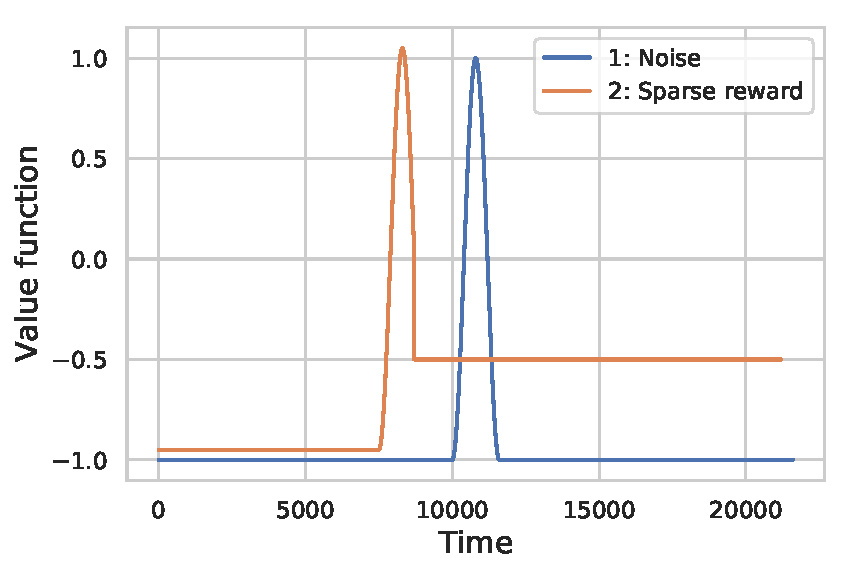
\includegraphics[scale=0.5]{fig/noise_sparse.pdf}
    \caption{Noise versus sparse reward}
    \label{fig:noise}
\end{figure}


\subsection{Adjusting for the reward}
In practice many environments in reinforcement learning have either a constant negative reward or a constant positive reward at every time step. In order to account for those rewards we propose an alternative formulation where $\vr$ accounts for the reward that was just seen:
\begin{equation}
\label{value_reward}
\begin{split}
    \vr(s_t) &= \param_t \Vt(s_t) + (1 - \param_t) (\vr(s_{t-1}) - r_{t-1}) \\ 
\end{split}
\end{equation}
The decision on the choice of formulation to use will depend on the environment considered. \comment{In the case where $\param$ is restricted to $\param = \{0,1\}$, the updates on a state $V(s_i)$ can be interpreted as an undiscounted N-step return:
\begin{equation}\label{undiscounted}
        \delta_t = V^{\pol}(s_t) + \sum_{p=i}^{t-1} r_p - \Vt(s_i).
\end{equation}}
From a theoretical perspective, convergence of this formulation can be considered by modifying the bound on $\Delta$ to accommodate the reward. This is left as a future work. 
\section{Related work}
Recurrent learning shares similarities with many algorithms in reinforcement learning. The most important similarity is with respect to $\lambda$ return \cite{sutton1998reinforcement,dayan1992convergence}. There is often a debate of explicit versus implicit modelling in reinforcement learning and supervised learning from a conceptual perspective. $\lambda$ return is a way to implicitly enforce temporal coherence through the trajectory. In this paper, we propose a method to \emph{explicitly} enforce the temporal coherence using recurrent learning. Furthermore, recurrent learning yields a natural way to estimate an emphasis function whereas setting $\lambda$ efficiently still remains an open problem. In practice both $\lambda$ return and recurrent learning may be needed to properly enforce temporal coherence. The capacity to ignore states also share some similar motivations to semi-Markov decision process \cite{puterman1990markov} and Temporal Value Transport \cite{TVT}. Temporal Value Transport attempts to exploit similar ideas that recurrent learning does. It does so in a different manner. In particular, Temporal Value Transport is based on a discrete attention mechanism using threshold values in contrast to our continuous $\param$ \emph{attention} mechanism. This yields very different algorithms and theory in practice. As mentioned earlier, there exists similarities with emphatic TD \cite{mahmood2015emphatic} in the sense that it emphasizes or de-emphasizes the update done to a state based on $\param$. One key difference with emphatic TD is that the interest is decayed across all the states using $\gamma$, whereas in this work it is based on the interest of the future states. Our formulation is driven by the success of \emph{forgetting} and \emph{ignoring} in supervised learning. Furthermore, learning the emphasis function is not explored in \cite{mahmood2015emphatic}. Our work also relates to Temporal Regularization \cite{thodoroff2018temporal} that smooth the target of temporal difference methods using previous values of the trajectory. Although sharing similar motivation, the algorithms proposed are different. In particular, learning \emph{smoothing} coefficient is not considered. Finally, \cite{xu2017natural} proposes a mechanism to adaptively learn to use previous estimates. In practice, this is done by considering an \emph{auxiliary loss} between the target and the previous estimate in contrast with the setup considered here. Furthermore, the theoretical properties(convergence) of their algorithm is not considered.


\comment{\subsection{Continuous time Markov + jump + all robotics event detection RNN and jumpy model}
\cite{feinberg2004continuous}
\cite{hochreiter1997long}}

\section{Experiments}
\begin{figure}[h]
    \centering
    \includegraphics[width=6cm]{fig/toy_MDP.png}
    \caption{Simple chain MDP. The dotted line in the figure indicates multiple states in between shown states.}
    \label{fig:toy MDP}
\end{figure}
We consider the simple chain MDP described in figure \ref{fig:toy MDP} to demonstrate our method. This MDP has three chains connected together to form a \emph{Y}. Each of the 3 chains (left of $S_1$, right of $S_2$, right of $S_3$) is made up of a sequence of states. The agent starts at $S_0$ and navigates through the chain. At the intersection, $S_1$, there is a $0.5$ probability to go top or bottom. The chain on the top has a reward of $+1$ at the last state and the chain on the bottom has a reward of $-1$. Every other transition has a reward of $0$, unless specified otherwise.\\
\subsection{Bias Variance trade-off}
\begin{figure}[h]
    \centering
    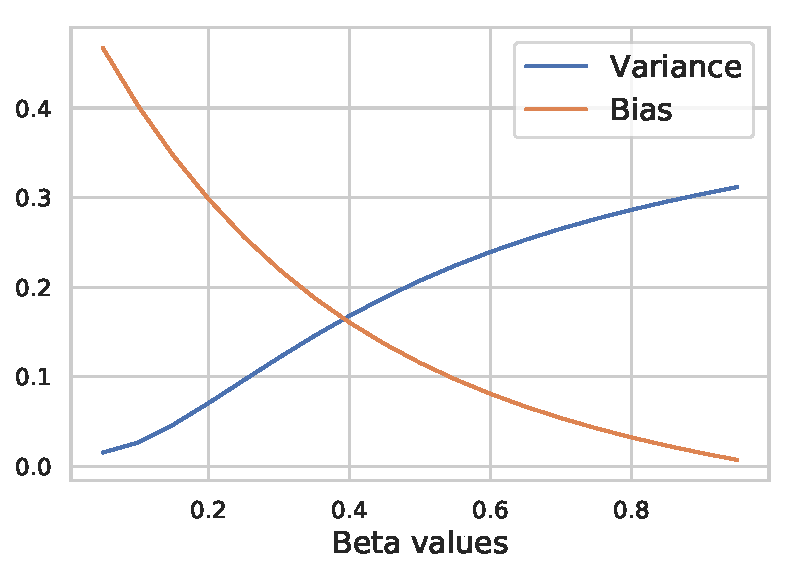
\includegraphics[scale=0.45]{fig/beta_bias_variance.pdf}
    \caption{Bias variance trade off of $\vr$ throughout the trajectory using exponential smoothing}
    \label{fig:bias_variance}
\end{figure}
It is possible to decompose policy evaluation into two sub tasks. The first one is given a set of functions $\Vt$, the goal is to estimate optimal values of states along the trajectory. The second task is to compare this set of functions that can be estimated by either considering the loss in Eq. \ref{simple_loss} or the recurrent loss in Eq. \ref{loss_beta}. In this experiment, we focus on the former task to demonstrate the bias variance trade-off induced by exponentially smoothing the values over the trajectory. This is shown in figure \ref{fig:bias_variance}. 
\begin{figure*}[t]
    \centering
    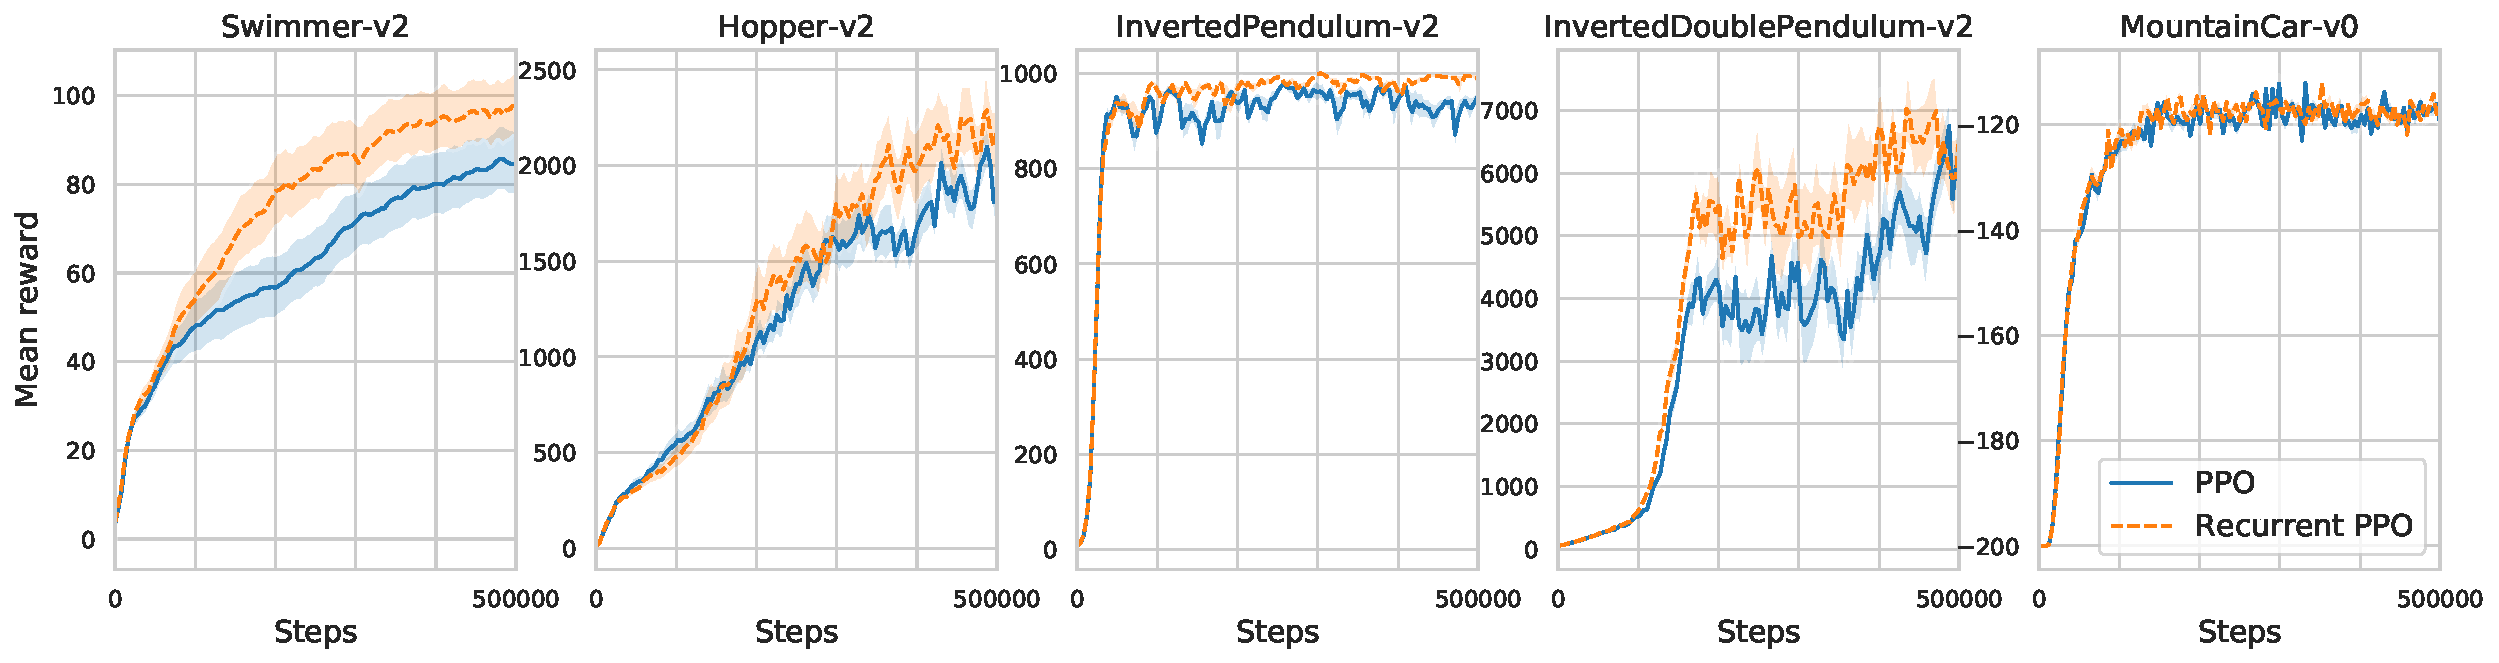
\includegraphics[scale=0.39]{fig/reward_mujoco.pdf}
    \caption{Performance on Mujoco environment. The X-axis represents the training steps and the Y-axis represents the mean reward}
    \label{fig:perf_mujoco}
\end{figure*}
The value function $\Vt$ is learned using TD(0) with the loss described in Eq. \ref{simple_loss}. For all states $s_i \in \mathbb{S}$ we average the bias and the variance of $\vr(s_i)$ over 500 episodes. We define the \emph{bias} as $\norm{\Vt(s_i) - \vr(s_i)}_{2}$. Intuitively, it is the distance between the estimate $\Vt(s_i)$(used as optimal values for this experiment) and the exponentially smoothed estimate $\vr(s_i)$. We experiment with a range of fixed $\param$'s. We observe a decrease in bias and an increase in the variance as the $\param$ increases. In other words, the value of each state is forced to be close to the values in the past when $\param$ is low. This results in smooth values along the trajectory but biased due to their reliance on the past. As $\param \to 1$ we tend to be close to classic TD setting. One important note, to accurately demonstrate the bias variance trade-off induced by using exponential smoothing, we use the same learning mechanism for both $\vr$ and $\Vt$, namely the loss in Eq. (\ref{simple_loss}). This choice is necessary to have a proper comparison; choosing different losses would induce different fixed points and make the comparison difficult.

\comment{\subsubsection{Bias reduction by learning $\param$ and including reward}
In this experiment TD outperforms both method but the aim is to showcase the learned beta}
\subsection{Partially observable setting}
\begin{figure}[h]
    \centering
    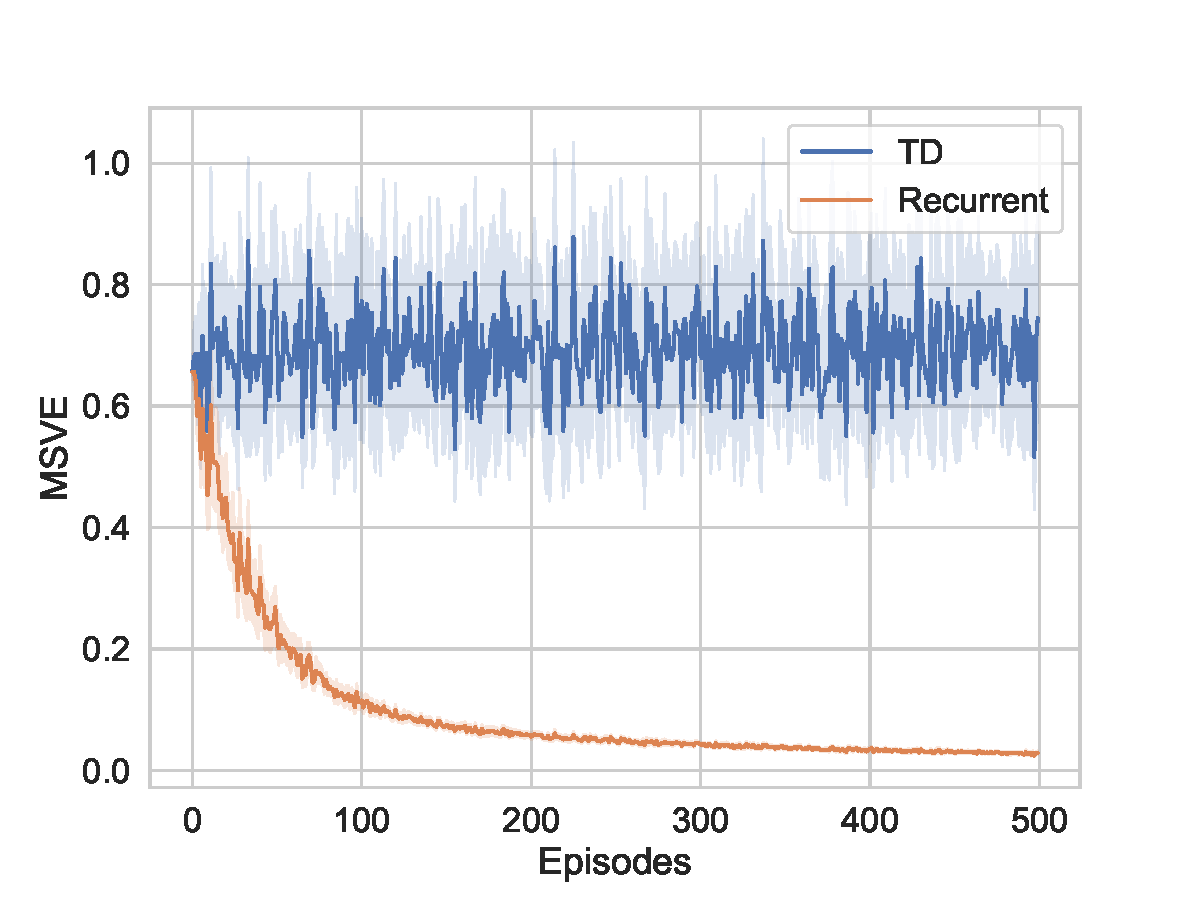
\includegraphics[scale=0.35]{fig/POMDP.pdf}
    \caption{TD versus Recurrent TD on aliased Y-chain}
    \label{fig:pomdp}
\end{figure}
Next, we explore the capacity of recurrent learning to solve a partially observable task. In particular, we consider the case where some states are aliased (share a common representation). The representation of the state following $S_4$ and $S_5$ in figure \ref{fig:toy MDP} is aliased. The goal of this environment is to correctly estimate the value of the aliased state $V^{\pol}(S_4)=0.81,V^{\pol}(S_5)=-0.81$(due to the discounting and the length of each chain being 5). When TD($\lambda$) is used to estimate the values for these states, the values of states $S_4$ and $S_5$ is close to 0 as the reward at the end of the chain is $+1$ and $-1$. However, when learning $\param$, recurrent learning achieve almost no error in the estimate of the aliased state as illustrated in figure \ref{fig:pomdp}. To understand this result the first thing to realize is that $\param=0$ on the aliased state as the previous values along the trajectory are a better estimate of the future along the same chain compared to the actual estimate of the aliased state. As $\param \to 0$, $\vr(S_4)$ and $\vr(S_5)$ tends to rely on the previous estimate $V(S_2)$ and $V(S_3)$ which are accurate. We see that learning to ignore certain states can sometimes be enough to solve correctly an aliased tasks in contrast to a traditional POMDP method that would attempt to infer the belief state. The results displayed in figure \ref{fig:pomdp} are averaged over 20 random seeds. The learning rate used is $0.05$, $\gamma = 0.9$ and $\lambda = 0.9$.
\subsection{Deep reinforcement learning}
\begin{figure*}[h]
    \centering
    \begin{minipage}[b]{0.17\linewidth}
    \centering
    
\includegraphics[width=\textwidth,height=2.8cm]{fig/phase_0.png}
    Phase 1: high $\param$
    \label{fig:phase_0}
    \end{minipage}
    \hspace{0.02cm}
    \begin{minipage}[b]{0.17\linewidth}
    \centering
    
\includegraphics[width=\textwidth,height=2.8cm]{fig/phase_1.png}
    Phase 2: low $\param$
    \label{fig:phase_1}
    \end{minipage}
    \hspace{0.02cm}
    \begin{minipage}[b]{0.17\linewidth}
    \centering
    
\includegraphics[width=\textwidth,height=2.8cm]{fig/phase_2.png}
    Phase 3: high $\param$
    \label{fig:phase_2}
    \end{minipage}
    \hspace{0.02cm}
    \begin{minipage}[b]{0.17\linewidth}
    \centering
    
\includegraphics[width=\textwidth,height=2.8cm]{fig/phase_3.png}
     Phase 4: low $\param$
    \label{fig:phase_3}
    \end{minipage}
    \hspace{0.02cm}
    \begin{minipage}[b]{0.17\linewidth}
    \centering
    
\includegraphics[width=\textwidth,height=2.8cm]{fig/phase_4.png}
    Phase 1: high $\param$
    \label{fig:phase_4}
    \end{minipage}
    \caption{Visual illustration of the cyclical behavior of $\param$ on Hopper}
    \label{fig:visual_hopper}
\end{figure*}

\begin{figure}[!h]
    \centering
    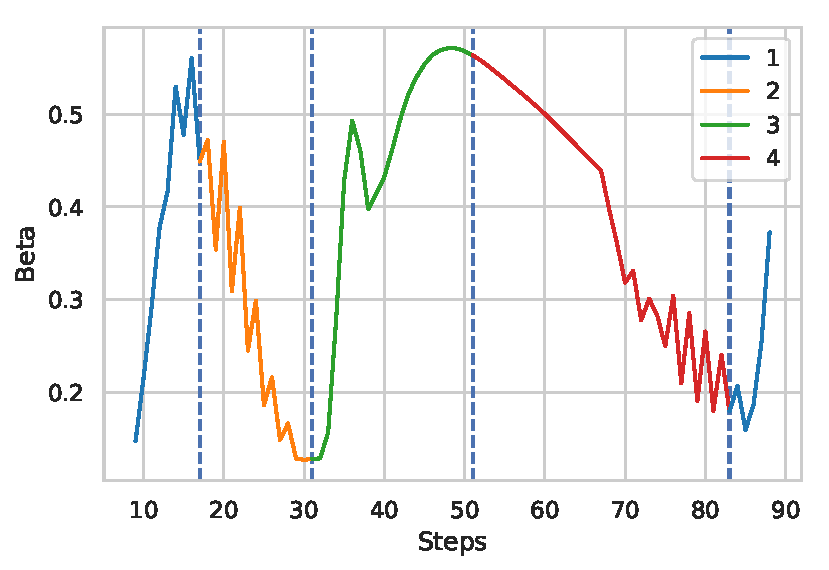
\includegraphics[scale=0.5]{fig/beta_hopper.pdf}
    \caption{Behavior of $\param$ through the trajectory on Hopper with the different phase described in figure $6$-$10$.}
    \label{fig:cyle_hopper}
\end{figure}

In this experiment, we modify the critic of Proximal Policy Optimization (PPO)~\cite{schulman2017proximal} to use recurrent learning. We modify the critic to estimate the value function parametrized by $\theta$ using recurrent learning. We add a separate network parametrized by $\omega$ (same architecture as PPO) to learn a state dependant $\param$. The following loss is minimized:
\begin{equation}\label{ppo_loss}
    \min_{\param,\omega} \expect_{\pol}(\Vt^{\lambda}-\vr)^2)
\end{equation}
where the target $\Vt^{\lambda}$ is the generalized advantage function \cite{schulman2015high}. Using an automatic differentiation library (Pytorch \cite{paszke2017automatic}) we differentiate Eq.\ref{ppo_loss} through the modified estimate to learn the $\theta$ and $\omega$. The hyperparameters of PPO are not modified. Due to the batch updates in PPO, obtaining the trajectory information to create the computational graph can be costly. As a result, we cut the backpropagation after $N$ timesteps in a similar manner to truncated backpropagation through time \cite{williams1995gradient}. The learning rate for the $\param$ network, L1 regularization coefficient of $\param$ and number of backpropagation steps were obtained using hyperparameter search and details can be found in the appendix \ref{deep_RL_appendix}. We used a truncated backprop of $N=5$ in our experiments as found no empirical improvements for $N=10$. However, we expect in some settings(e.g. long term credit assignment) backprop further can be advantageous. The motivation to regularize $\param$ to be sparse comes from bounded rationality. Our brain has limited capacity and only updating the value at key states is a desirable property. This parameter plays a similar role as the deliberation cost in option \cite{harb2018waiting}. The best performing set of parameters included a regularization parameter of $0.5$ supporting this hypothesis. The performance reported are averaged over 20 different random seeds. \footnote{The base code used to develop this algorithm can be found here \cite{pytorchrl}. The code for Recurrent PPO can be found in the supplementary material}.

 
\subsubsection{Performance}
The algorithm was tested on seven different games of the Mujoco suite \cite{todorov2012mujoco}. As demonstrated in the figure \ref{fig:perf_mujoco}, we observe an increase in performance on four of the tasks (Swimmer, Hopper, Inverted Pendulum, Double Inverted Pendulum). The performances are averaged over 20 seeds and a confidence interval of $95\%$ is used. For the other three tasks (Half Cheetah, Walker, Mountain Car) the performances were found to be comparable. The performance graphs for all the games can be found in figure \ref{fig:full_mujoco} in the appendix. The mean beta values and variance for all the tasks can also be found in the appendix (figure \ref{fig:beta_mean},\ref{fig:beta_std}).
One interesting finding in the figure \ref{fig:perf_mujoco} concerns inverted-pendulum in the context of generalization. Though the convergence is quick for PPO, severe performance drops (reward drop by more than $100$) can be observed. We found that recurrent learning stabilizes the learning and suffer significantly less drops during training. We notice that on an average PPO will suffer from 5.91 drops below 900 points over 500k steps. In contrast, recurrent learning will only drop 3.53 times. This represent a 40\% drop in \emph{catastrophic forgetting} underlying the potential robustness of recurrent learning.

\subsubsection{Qualitative interpretation of $\param$ }

\emph{Hopper}: At the end of training, we qualitatively analyze $\param$ through the trajectory and observe the cyclical behavior shown in figure \ref{fig:cyle_hopper}, where different colors describe various stages of the cycle. One intuitive way to look at $\param$ is: \emph{if I were to give a different value to a state would that alter my policy significantly?} We observe an increase in $\param$ value when the agent has to take an important decision like jumping or landing. We see a decrease in $\param$ when the agent has trivial actions to perform. This pattern is illustrated in the figure \ref{fig:visual_hopper} and \ref{fig:cyle_hopper}. This behaviour is cyclic and repetitive and a video of the same can be found at the following link\footnote{\url{https://youtu.be/0bzEcrxNwRw}{}}. One surprising fact was that this behavior was obtained without any regularization on $\param$. Similar behavior can be observed with regularization although the mean and variance of $\param$ diminishes.\\
 \begin{figure}[]
     \centering
     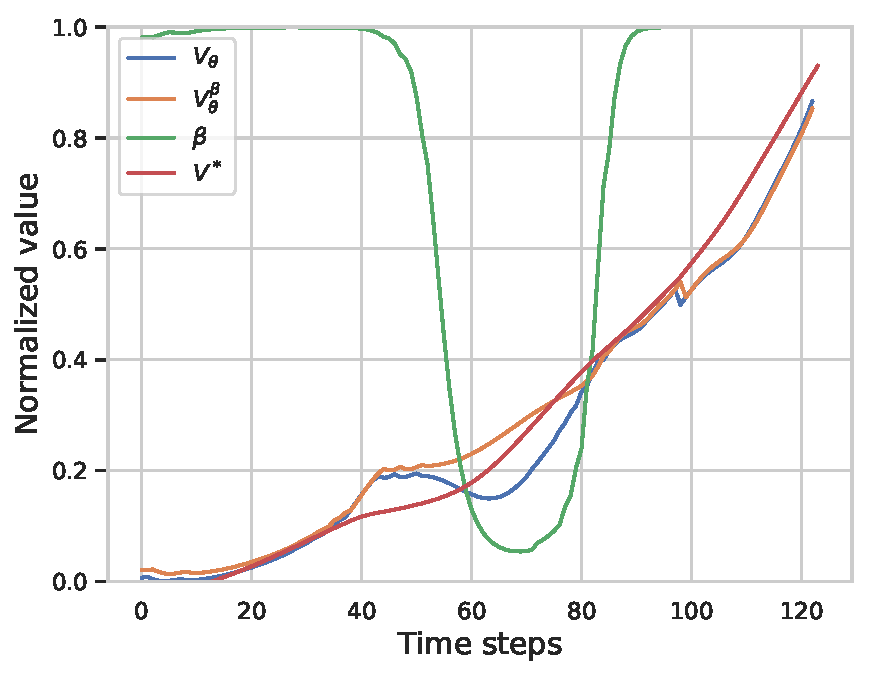
\includegraphics[scale=0.45]{fig/mountain.pdf}
     \caption{Behavior of $\param$ and the value function on Mountain-Car}
     \label{fig:my_label}\label{mountain_car}
 \end{figure}
\emph{Mountain car}: Two scenarios may happen when the agent is climbing up the hill on the right side. Either the agent has enough velocity to finish the game and obtain a high reward, or it doesn't have enough velocity and goes back down the hill. During early stages of training, the function approximator is confused about the scenarios mentioned earlier, resulting a drop in value function around step 100 as shown in figure \ref{mountain_car}. The value increases again once the agent climbs the hill with more velocity. In PPO, we can obtain a more accurate target by setting $\tau$ to a high value, thereby eliminating a drop in value. This enables the $\param$ network to learn to trust its past estimate rather than the noisy point estimate, hence a significant drop in the $\param$ value. As a result, $\vr$ becomes a  better estimate of the target than $\Vt$ in this scenario. After training PPO for a while this drop disappears and the $\param$ mean goes to 1. This experiment shows the potential of $\param$ to smooth out noisy estimates in the trajectory. One caveat to consider is the feedback loop induced by ignoring a state in control. When the policy changes a state that can be ignored at the beginning may be essential later on. One way to address this is to avoid saturating $\param$ such that learning remains possible later on.


\section{Discussions}
\paragraph{$\param$ as an interest function:} One interesting result of this work is that the $\param$ network learns to ignore some state without any restrictions imposed on it. It does so in order to reduce the variance. Furthermore, this $\param$ can be interpreted as an \emph{interest} function. In reinforcement learning, having access to a function quantifying the \emph{interest} \cite{mahmood2015emphatic} of a state can be helpful. For example, one could decide to explore from those states, prioritize experience replay based on those states. Further work can be done to study how $\param$ may impact performance. We also believe $\param$ can be related to the concepts of bottleneck state \cite{tishby2011information}. Finally, the concept of interest state in recurrent learning aligns well with the notion of interest state for the $\lambda$ return. Indeed bootstrapping on states with similar values than the one estimated will only result in variance. The most informative updates comes from bootstrapping on state with different value. 

\paragraph{Partial observability:} As demonstrated in the experiments earlier, recurrent learning is able in some cases to correctly estimate the value of aliased state using trajectory's estimate. This is a promising area to research as the experiments suggest that ignoring an uninformative state can sometimes be enough to learn its value function. This is in contrast to traditional POMDP method that attempts to infer the belief state. Inferring the true underlying state is not always feasible. In some cases learning to ignore aliased state and relying on previous estimates may be an easier task.
\comment{\paragraph{Relationship between $\lambda$ and $\param$:} There exists an important relationship between $\lambda$ and $\param$. $\param$ can choose to ignore a state if the past is different from the future. We could get a better estimate of the future using $\lambda$ returns when compared against one step methods. Hence, a need for long horizon to learn accurate $\param$. This behaviour can also be seen in our \emph{mountain car} experiment. Also, bootstrapping from states that are ignored would be detrimental to the learning process. A state is never updated if it has $\param=0$ hence bootstrapping from this state will induce \emph{wrong} bias. To avoid this issue, one approach could be to use learned $\param$ as a state dependent $\lambda$ hence making correct updates.}
\paragraph{Asymptotic convergence:} As mentioned previously assumption 2 is too restrictive to guarantee convergence in all tabular settings. This analysis could be refined by considering the trajectory's information to bound $\Delta$. As an example, one could consider any physical system where transition in the state space are smooth (continuous state space) and bounded by some Lipschitz constant in a similar manner than \cite{shah2018q}. 
\paragraph{Bias of the eligibility trace:}
We showed in Eq. \eqref{trace} a technique to compute the gradient of the estimate recursively. This technique is computationally inexpensive compared to the recursive backpropogation as the gradient from the past is accumulated. But this kind of an update is biased. This bias comes from the fact that the true gradient obtained by applying the chain rule at future step is different than the trace if the parameters are updated at each time step. This is a similar problem encountered by eligibility traces \cite{seijen2014true} and real time recurrent learning \cite{williams1995gradient}. Similar idea than \cite{seijen2014true} may be used to obtain an unbiased estimate.
\paragraph{Recurrent learning for action:} We have not explored the concept of recurrent learning for actions (Q values and policy gradient). This is a promising area as constraining actions to be temporally coherent is a natural prior to induce on a function approximator. This technique could also be interesting in the context of exploration as this could yield a \emph{structured exploration}. Finally, this framework with learning $\param$ can be cast as a \emph{vanilla} version of options \cite{sutton1999between}. 

%Another important similarity is with \cite{mahmood2015emphatic} in which ideas such as emphasizing the states and limited capacity of a network are explored. But in this work, the estimate in the update equation depends on the previous value functions which is not the case in \cite{mahmood2015emphatic}. Our formulation helps in accurate credit assignment when we set the $\param$ correctly. This aspect is not investigated in this work and can be explored further. Another aspect we found in our initial experimentation that can be explored further is generalization. We believe learning $\param$ would help in generalization of tasks in reinforcement learning.

\paragraph{Conclusion:}This paper proposes a technique to address two important aspects of reinforcement learning algorithms namely - temporal coherence, and selective updating. First, we prove asymptotic convergence of the proposed method. Later, we provide a bias-variance argument to emphasize the importance of temporal coherence. Then, we demonstrate interesting properties that result while we emphasize and de-emphasize updates on states during learning. We provide experiments to corroborate the application of our method in a partially observable domain and for continuous control.





